\documentclass{article} 

\usepackage[utf8]{inputenc}
\usepackage{amsmath, amssymb}
\usepackage{graphicx}
\usepackage{booktabs} 
\usepackage{geometry}
\usepackage{float}
\usepackage{hyperref}
\usepackage{listings}
\usepackage{xcolor}
\usepackage{tabularx}
\usepackage{seqsplit}
\usepackage{multirow} 
\usepackage{algorithm}
\usepackage{algorithmic}
\usepackage{subcaption}

\geometry{a4paper, margin=1in}

\renewcommand{\thefigure}{S\arabic{figure}}
\renewcommand{\thetable}{S\arabic{table}}
\renewcommand{\thesection}{S\arabic{section}}
\renewcommand{\theequation}{S\arabic{equation}}

\setcounter{figure}{0}
\setcounter{table}{0}
\setcounter{section}{0}
\setcounter{equation}{0}

\title{\textbf{Supplementary Material for:}\\ \Large MZSGO: multimodal zero-shot protein function annotation via evolutionary signals and textual semantics}
\author{Boyue Cui, Yujuan Li, Shiqu Chen,Jiaming Wei, Xuan Wang, Yadong Wang, Junyi Li}
\date{}

\begin{document}

\maketitle

\section{Impact of Joint Training on Model Performance}

To validate the hypothesis that training all Gene Ontology (GO) domains jointly compromises the model's capacity to learn features unique to each ontology, we conducted a comparative experiment. We evaluated two architectures, ProtNote and our proposed MZSGO, under two distinct training strategies:
\begin{enumerate}
    \item \textbf{Separate Training:} Models are trained specifically for a single ontology (Biological Process, BP; Molecular Function, MF; and Cellular Component, CC).
    \item \textbf{Unified Training:} A single model is trained jointly on all three ontologies simultaneously.
\end{enumerate}

Figure S1 illustrates the performance comparison in terms of Fmax scores. As observed, the unified training strategy consistently underperformed the separate training strategy across all ontologies and model architectures. 

\begin{figure}[h]
    \centering
    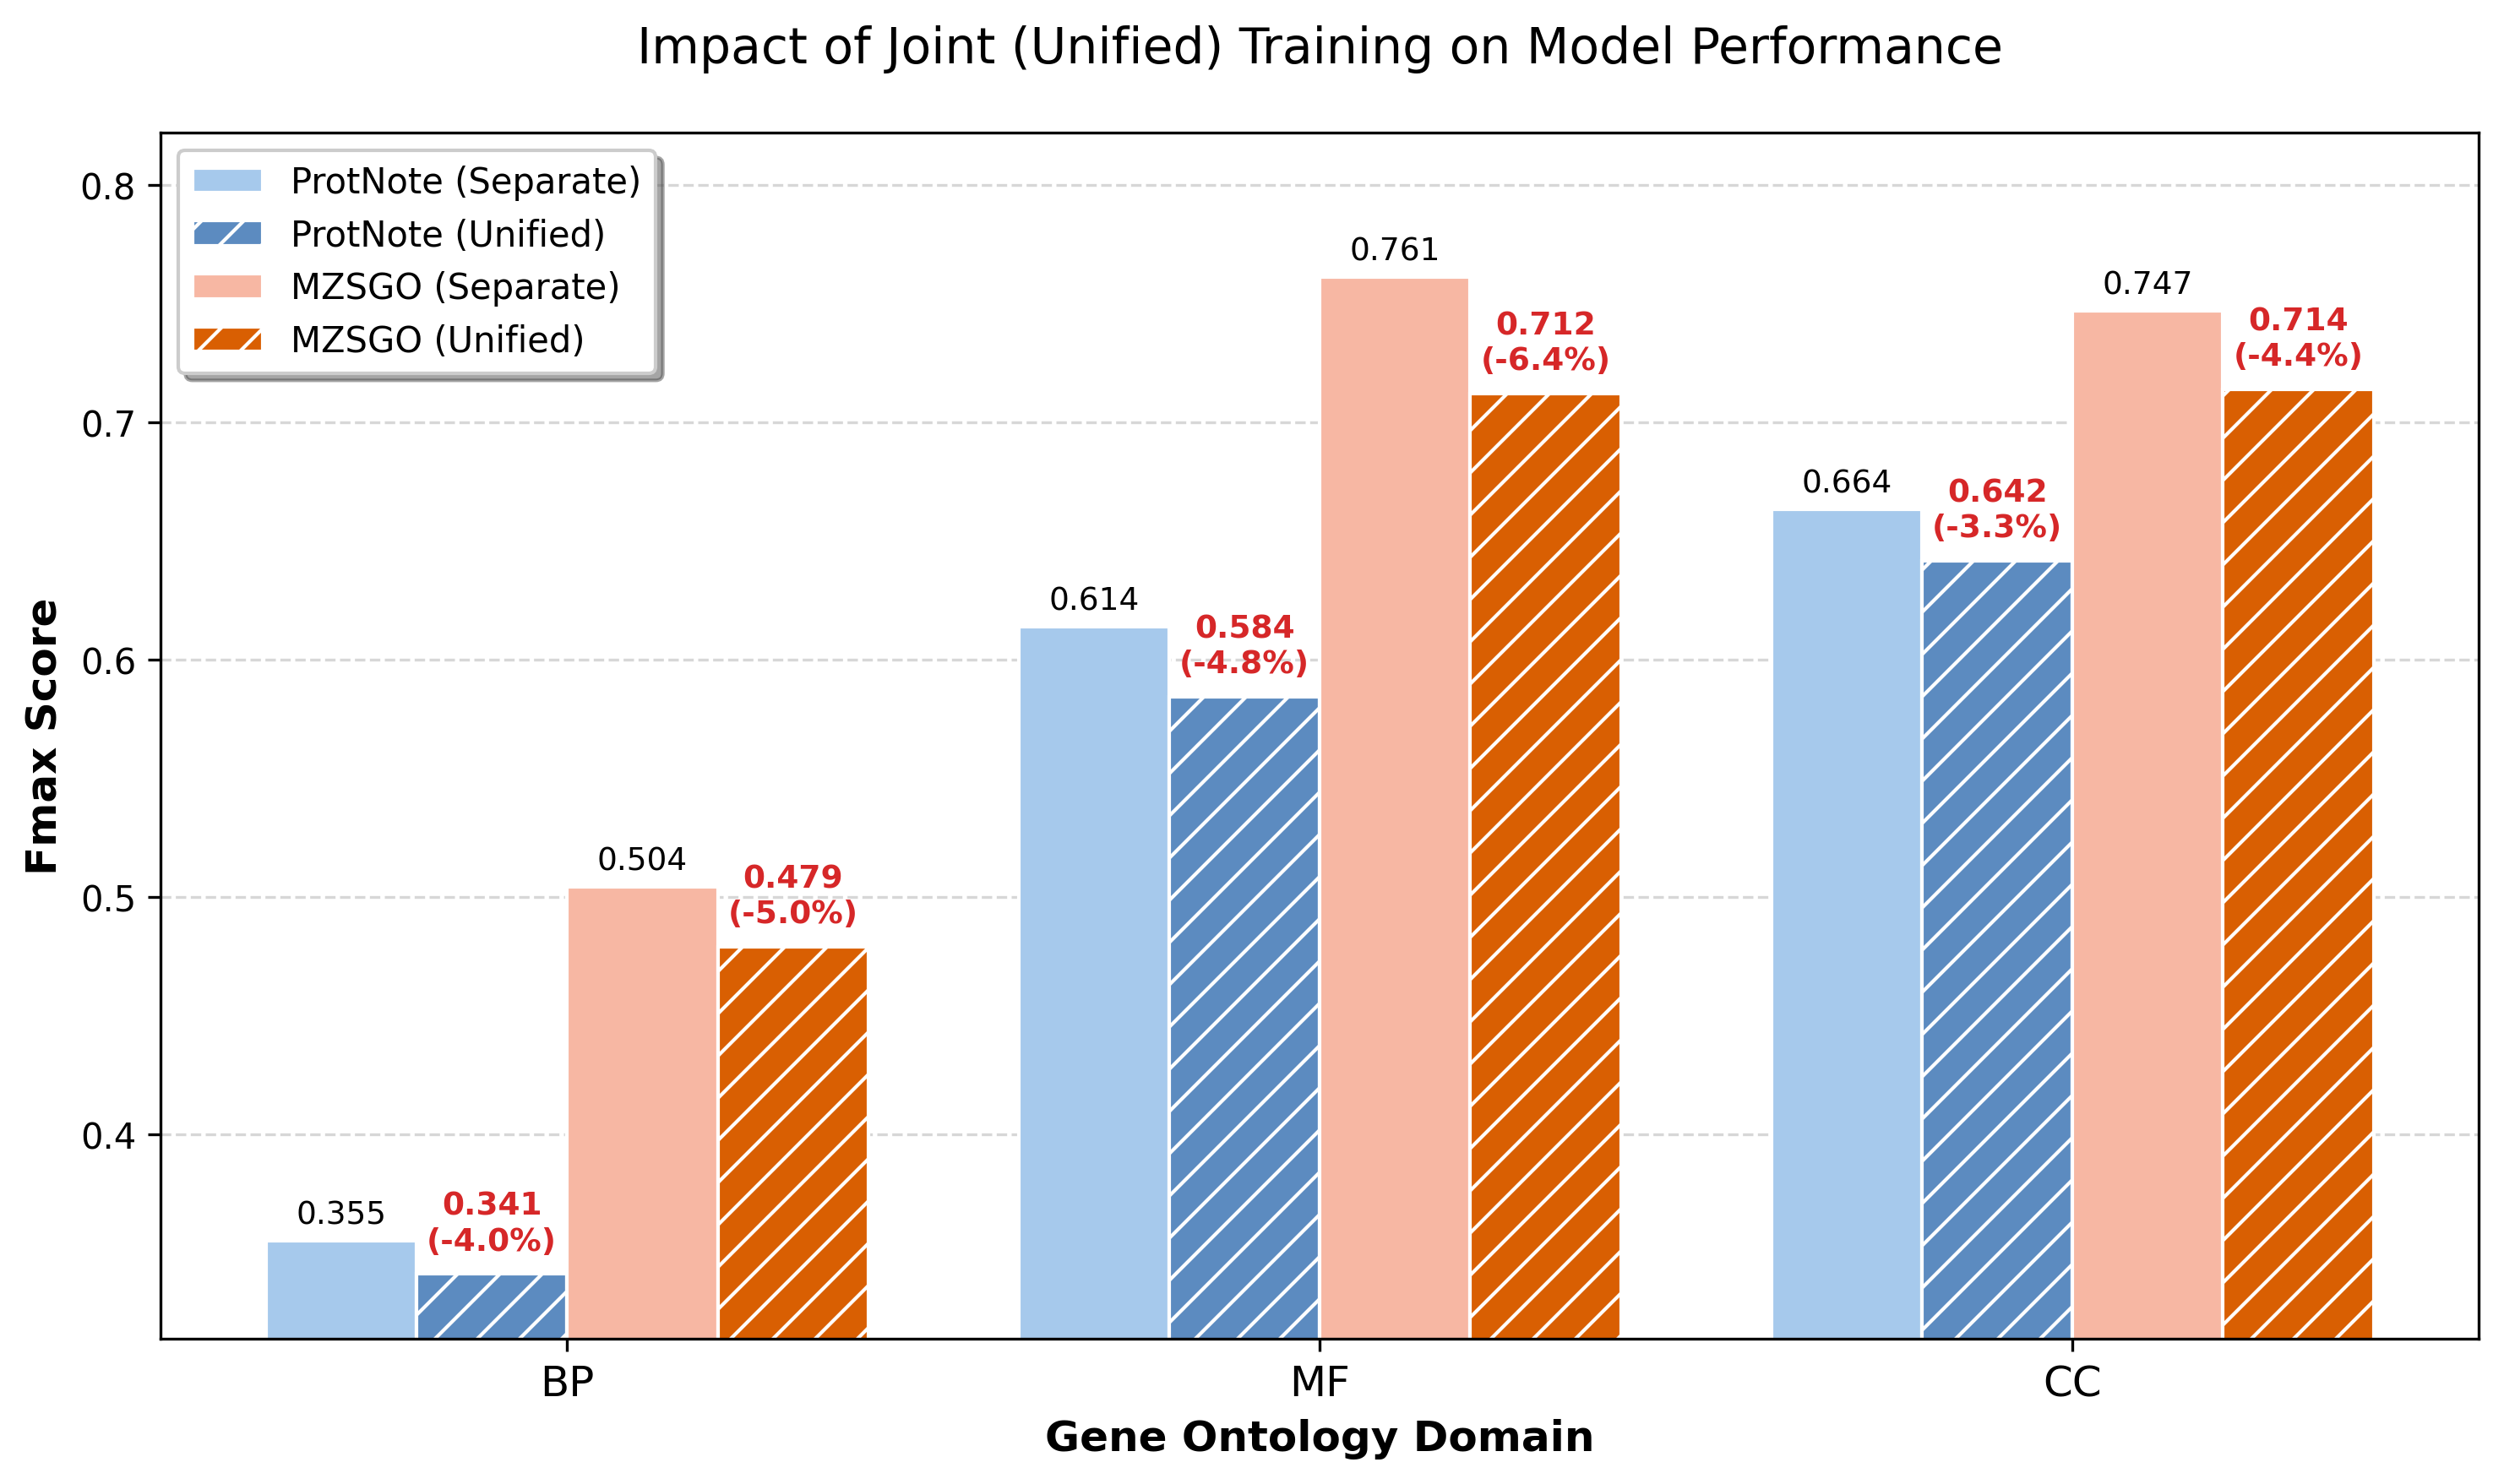
\includegraphics[width=0.7\linewidth]{picture/unified_vs_separate.png}
    \caption{Comparison of Fmax scores between separate and unified training strategies.}
    \label{fig:supp_ablation}
\end{figure}

\section{Comparative Results without Training Set Filtering}
\label{supp:s3}

The complete CAFA5 training set within the Swiss-Prot database comprises 72,390 entries. We observed that when the full training set is utilized—which inevitably includes proteins unlabeled for a specific target ontology category—most baseline methods are negatively affected by these implicit "negative" samples, leading to suboptimal performance.

In contrast, methods that cast the protein function task as a binary classification problem (such as ProtNote and our method, MZSGO) demonstrate robustness on the full, unfiltered dataset without significant performance degradation. Figure \ref{fig:ontology_comparison} presents the comparative experimental results without training set filtering. As shown, MZSGO consistently outperforms the latest baselines (ProtGO, DpFunc, and ProtNote) across all three ontology categories in both Fmax and AUPR metrics.

\begin{figure}[htbp]
    \centering
    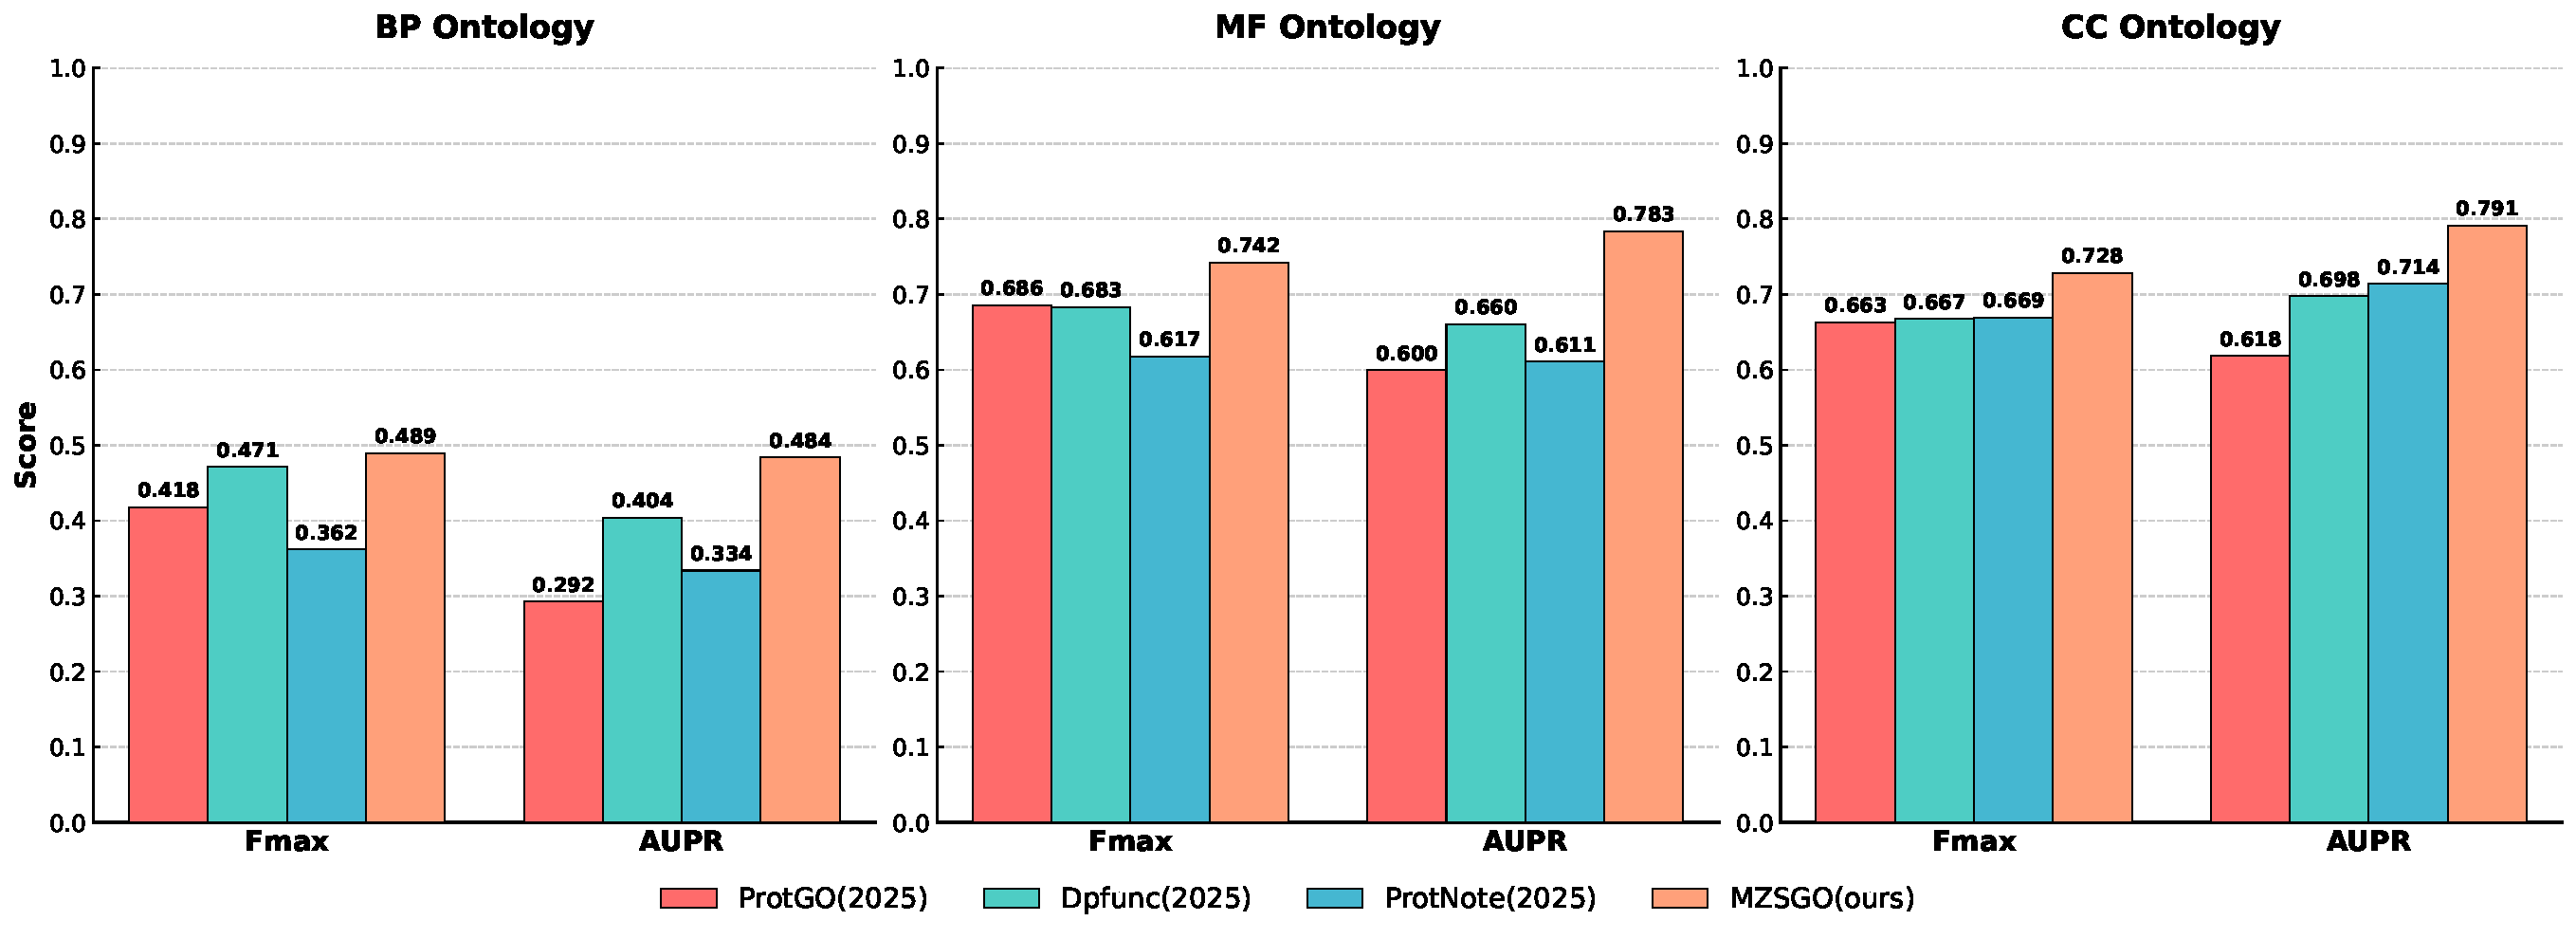
\includegraphics[width=\textwidth]{picture/ontology_comparison.pdf}
    \caption{Performance comparison of MZSGO with state-of-the-art methods on the full, unfiltered training set. The evaluation metrics (F-max and AUPR) are reported for BP, MF, and CC ontologies. Our method demonstrates superior performance across all metrics.}
    \label{fig:ontology_comparison}
\end{figure}

\newpage
\section{Example Input Data}
\label{supp:s1}

This section presents a complete example of the input data for a single protein entry (UniProt ID: Q8TBH0). Table \ref{tab:example_data} consists of three modalities: the raw amino acid sequence, domain text descriptions derived from InterPro, and candidate GO term definitions (showing positive samples).

\begin{table}[htbp]
    \centering
    \caption{An example input data structure for Protein Q8TBH0.}
    \label{tab:example_data}
    \renewcommand{\arraystretch}{1.4} 
    \small 
    
    \begin{tabularx}{\textwidth}{@{} p{2.5cm} >{\raggedright\arraybackslash}X @{}}
        \toprule
        \textbf{Data Modality} & \textbf{Content} \\
        \midrule
        \textbf{Entry ID} & Q8TBH0 \\
        \midrule
        
        \textbf{Modality 1:}\newline Protein Sequence & 
        \texttt{\seqsplit{MLFDKVKAFSVQLDGATAGVEPVFSGGQAVAGRVLLELSSAARVGALRLRARGRAHVHWTESRSAGSSTAYTQSYSERVEVVSHRATLLAPDTGETTTLPPGRHEFLFSFQLPPTLVTSFEGKHGSVRYCIKATLHRPWVPARRARKVFTVIEPVDINTPALLAPQAGAREKVARSWYCNRGLVSLSAKIDRKGYTPGEVIPVFAEIDNGSTRPVLPRAAVVQTQTFMARGARKQKRAVVASLAGEPVGPGQRALWQGRALRIPPVGPSILHCRVLHVDYALKVCVDIPGTSKLLLELPLVIGTIPLHPFGSRSSSVGSHASFLLDWRLGALPERPEAPPEYSEVVADTEEAALGQSPFPLPQDPDMSLEGPFFAYIQEFRYRPPPLYSEEDPNPLLGDMRPRCMTC}} \\
        \midrule
        
        \textbf{Modality 2:}\newline Domain Text Descriptions & 
        $\bullet$ IPR011021: Domain: Arrestin-like, N-terminal \newline
        $\bullet$ IPR011022: Domain:Arrestin: C-terminal-like domain \newline
        $\bullet$ IPR014752: Homologous\_superfamily: Arrestin-like, C-terminal \newline
        $\bullet$ IPR014756: Homologous\_superfamily: Immunoglobulin E-set \newline
        $\bullet$ IPR050357: Family: Arrestin domain-containing protein \\
        \midrule
        
        \textbf{Modality 3:}\newline GO Term Descriptions \newline (positive samples) & 
        \textbf{GO:0005622  } \newline
        intracellular anatomical structure: A component of a cell contained within (but not including) the plasma membrane. In eukaryotes it includes the nucleus and cytoplasm. \vspace{1.5ex} \newline
        
        \textbf{GO:0043226  } \newline
        organelle: Organized structure of distinctive morphology and function. Includes the nucleus, mitochondria, plastids, vacuoles, vesicles, ribosomes and the cytoskeleton. Excludes the plasma membrane. \vspace{1.5ex} \newline
        
        \textbf{GO:0005575 } \newline
        cellular\_component: A location, relative to cellular compartments and structures, occupied by a macromolecular machine when it carries out a molecular function. \vspace{1.5ex} \newline
        
        \textbf{GO:0016020} \newline
        membrane: A lipid bilayer along with all the proteins and protein complexes embedded in it and attached to it. \\
        \bottomrule
    \end{tabularx}
\end{table}

\section{Algorithm Pseudo-code}
The detailed training procedure for the MZSGO framework is outlined in Algorithm \ref{alg:mzsgo}.

\begin{algorithm}
\caption{MZSGO Workflow}
\label{alg:mzsgo}
\begin{algorithmic}[1]

\REQUIRE $E_{esm}, E_{dom}$ (protein features), $E_{nlp}$ (label features)

\ENSURE Prediction Matrix $Y \in \mathbb{R}^{B \times L}$

\STATE \textbf{Define} $\phi(\cdot)$: Generic MLP block (Linear $\to$ LN $\to$ Act $\to$ Dropout)

\vspace{0.1cm}
\STATE \COMMENT{\textbf{1. Projection \& Alignment}}
\STATE Project features to hidden dimension  $H$:
\STATE $\mathbf{h}_{esm} \leftarrow \phi_{1}(E_{esm}), \quad \mathbf{h}_{dom} \leftarrow \phi_{2}(E_{dom}), \quad \mathbf{h}_{nlp} \leftarrow \phi_{3}(E_{nlp})$
\STATE Broadcast features to shape $[B \cdot L, H]$ to form protein–label pairs:
\STATE $\mathbf{H} \leftarrow \{ \mathbf{h}_{dom}^{expand}, \mathbf{h}_{esm}^{expand}, \mathbf{h}_{nlp}^{expand} \}$

\vspace{0.1cm}
\STATE \COMMENT{\textbf{2. Feature Dropout (Training Only)}}
\IF{Training}
\STATE Generate mask $M \in \{0,1\}^{B \cdot L \times 2}$ s.t. at least one protein feature is kept per row.
\STATE $\mathbf{h}_{dom}^{expand} \leftarrow \mathbf{h}_{dom}^{expand} \odot M_{:,0}$
\STATE $\mathbf{h}_{esm}^{expand} \leftarrow \mathbf{h}_{esm}^{expand} \odot M_{:,1}$
\ENDIF

\vspace{0.1cm}
\STATE \COMMENT{\textbf{3. Gated Fusion}}
\STATE Concatenate all modalities: $\mathbf{Z}_{cat} \leftarrow \text{Concat}(\mathbf{H}, \text{dim}=-1)$
\STATE Compute Gate Weights (Attention):
\STATE $\mathbf{W} \leftarrow \text{Softmax}(\phi_{gate}(\mathbf{Z}_{cat})) \quad \triangleright \text{Shape: } [B \cdot L, 3]$
\STATE Weighted Sum Fusion:
\STATE $\mathbf{F}_{fused} \leftarrow \sum_{k=1}^{3} \mathbf{W}_{:,k} \cdot \phi_{trans}(\mathbf{H}_k)$

\vspace{0.1cm}
\STATE \COMMENT{\textbf{4. Classification}}
\STATE $Y \leftarrow \text{Reshape}(\text{Linear}(\phi_{cls}(\mathbf{F}_{fused})), [B, L])$

\RETURN $Y$

\end{algorithmic}
\end{algorithm}

\section{Statistical Rationale for Loss Function Selection}

To determine the optimal optimization objectives for BP, MF, and CC, we analyzed their label distributions using the Gini Coefficient (inequality) and Effectiveness Ratio (redundancy).

\subsection{Metric Definitions}

\paragraph{Gini Coefficient ($G$)}
This metric quantifies distributional inequality. Let $x$ be the label counts sorted in non-decreasing order ($x_1 \le \dots \le x_C$). The coefficient is computed as:
\begin{equation}
    G = \frac{2 \sum_{i=1}^C i \cdot x_i}{C \sum_{i=1}^C x_i} - \frac{C+1}{C}
\end{equation}
$G \approx 1$ implies maximal inequality, where a few "head" classes dominate the dataset.

\paragraph{Effectiveness Ratio ($\rho$)}
Following \cite{cui2019class}, the marginal benefit of adding samples diminishes due to information overlap. The effective number for a class with $n$ samples is $E_n = (1 - \beta^n)/(1 - \beta)$, with $\beta = 0.9999$. We define $\rho$ as the ratio of the mean effective count to the mean actual count:
\begin{equation}
    \rho = \frac{\frac{1}{C}\sum_{i=1}^C E_{n_i}}{\frac{1}{C}\sum_{i=1}^C n_i}
\end{equation}
A lower $\rho$ indicates high redundancy, where gradients are dominated by repetitive examples.

\subsection{Analysis and Selection}

MF and BP exhibit relatively high information quality, with Effectiveness Ratios of 72.20\% and 81.11\%, respectively. This suggests that despite inherent imbalance, the positive samples provide sufficient unique gradients. Consequently, we employ standard Binary Cross-Entropy (BCE) for these branches.

In contrast, CC demonstrates extreme inequality ($G=0.946$) and the lowest Effectiveness Ratio (57.60\%), significantly worse than BP or MF. This indicates that nearly half of the CC sample volume contributes minimal marginal information. Standard BCE would allow these frequent, redundant examples to overwhelm the learning process. Therefore, we utilize Focal Loss specifically for CC to down-weight easy examples and focus on informative tail classes.

\begin{figure}[h]
    \centering
    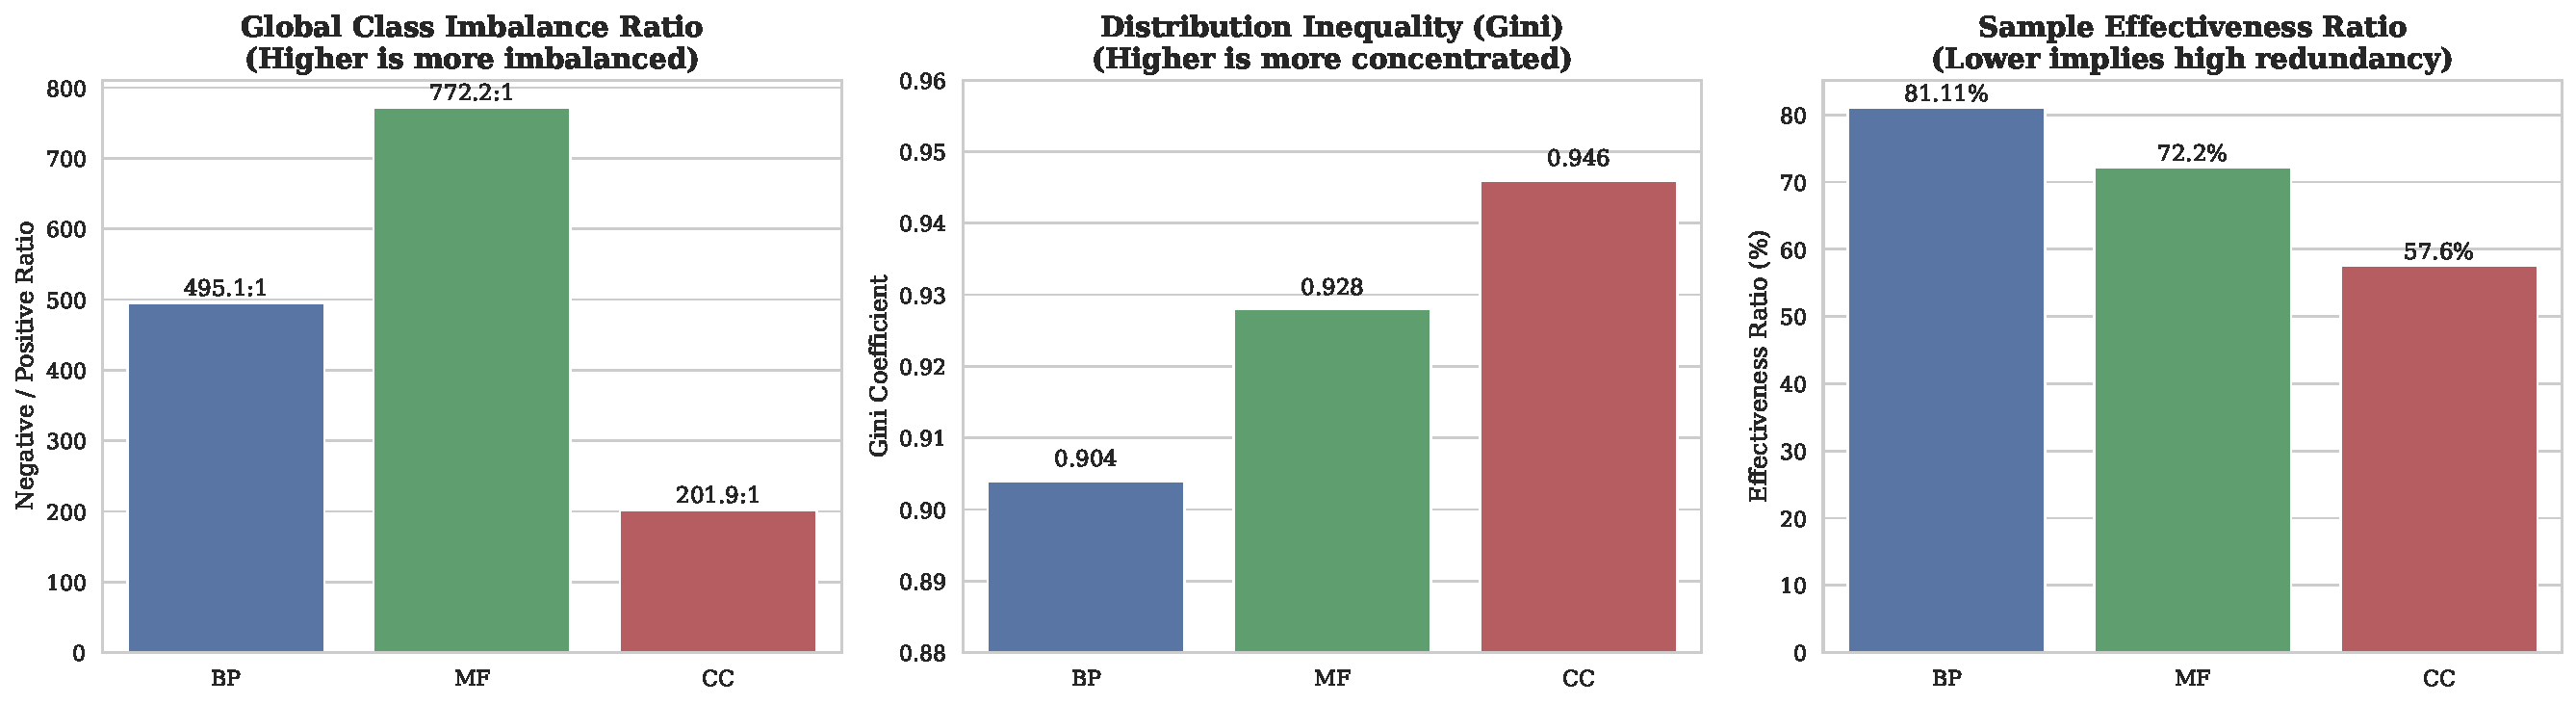
\includegraphics[width=1\linewidth]{picture/loss_selection_analysis.pdf}
    \caption{Statistical comparison justifying loss function selection. CC shows the highest inequality and lowest effectiveness, necessitating Focal Loss.}
    \label{fig:loss_analysis}
\end{figure}

\section{Detailed Evaluation Metrics}
\label{supp:metrics}

In this section, we provide the mathematical definitions of the evaluation metrics used in our study. Following the standard protocols of the CAFA challenge, we employ protein-centric metrics to evaluate the performance of multi-label protein function prediction.

Let $N$ be the total number of protein sequences in the test set. For a given protein $i$, let $T_i$ be the set of ground truth GO terms (true labels), and let $P_i(t)$ be the set of predicted GO terms with a confidence score greater than or equal to a threshold $t \in [0, 1]$.

\subsection{Standard Protein-centric Metrics}

\subsubsection{Precision and Recall}
For a specific threshold $t$, the precision ($\pi_i(t)$) and recall ($\rho_i(t)$) for the $i$-th protein are defined as:

\begin{equation}
    \pi_i(t) = \frac{|P_i(t) \cap T_i|}{|P_i(t)|}, \quad \rho_i(t) = \frac{|P_i(t) \cap T_i|}{|T_i|}
\end{equation}

where $|\cdot|$ denotes the size of the set. The average precision ($AvgPr(t)$) and average recall ($AvgRc(t)$) across the dataset are calculated as:

\begin{equation}
    AvgPr(t) = \frac{1}{M(t)} \sum_{i=1}^{N} \pi_i(t) \cdot \mathbb{I}(|P_i(t)| > 0)
\end{equation}

\begin{equation}
    AvgRc(t) = \frac{1}{N} \sum_{i=1}^{N} \rho_i(t)
\end{equation}

Here, $M(t)$ represents the number of proteins with at least one prediction at threshold $t$.

\subsubsection{F-max}
The $F_{max}$ score is the maximum harmonic mean of average precision and average recall calculated over all possible thresholds $t$:

\begin{equation}
    F_{max} = \max_{t \in [0, 1]} \left( \frac{2 \cdot AvgPr(t) \cdot AvgRc(t)}{AvgPr(t) + AvgRc(t)} \right)
\end{equation}

\subsubsection{Area Under the Precision-Recall Curve (AUPR)}
AUPR is calculated by integrating the precision-recall curve:

\begin{equation}
    AUPR = \int_{0}^{1} AvgPr(Rc) \, d(AvgRc)
\end{equation}

Note that in our evaluation protocol, AUPR is computed on protein-centric precision–recall curves over the full label space. Even for models that assign zero scores to unseen labels, the curve still contains non-zero precision–recall points (e.g., at threshold 0). As a result, the numerical AUPR is slightly above zero, although the model has no effective discriminative ability for unseen labels.

\subsection{Generalized Zero-Shot Metrics}

To evaluate the model's generalization capability, we split the label space into seen classes ($L_{seen}$) and unseen classes ($L_{unseen}$). We calculate the AUPR separately for these subsets:

\begin{itemize}
    \item \textbf{Seen AUPR}: Calculated by restricting the evaluation to the subset of labels present in the training set.
    \item \textbf{Unseen AUPR}: Calculated by restricting the evaluation to the subset of labels never encountered during training.
\end{itemize}

To assess the trade-off between fitting known knowledge and generalizing to new concepts, we compute the Harmonic Mean ($H$) of these two metrics:

\begin{equation}
    H = \frac{2 \cdot \text{AUPR}_{seen} \cdot \text{AUPR}_{unseen}}{\text{AUPR}_{seen} + \text{AUPR}_{unseen}}
\end{equation}

A high $H$ score indicates that the model achieves a balanced performance, avoiding the common pitfall of overfitting to seen classes while failing on unseen ones.

\subsection{Weighted Evaluation Metrics}

To account for the varying specificity of GO terms, we employ weighted metrics where each term $v$ is assigned a weight $\tau(v)$ based on its Information Content (IC). The IC is typically defined as $\tau(v) = -\log(p(v))$, where $p(v)$ is the probability of term $v$ occurring in the database.

\subsubsection{Weighted Precision and Recall}
For a protein $i$ at threshold $t$, the weighted precision $w\pi_i(t)$ and weighted recall $w\rho_i(t)$ are:

\begin{equation}
    w\pi_i(t) = \frac{\sum_{v \in P_i(t) \cap T_i} \tau(v)}{\sum_{v \in P_i(t)} \tau(v)}, \quad w\rho_i(t) = \frac{\sum_{v \in P_i(t) \cap T_i} \tau(v)}{\sum_{v \in T_i} \tau(v)}
\end{equation}

\subsubsection{Weighted F-max ($wF_{max}$) and Weighted AUPR ($wAUPR$)}
Similar to the standard metrics, $wF_{max}$ is the maximum harmonic mean of the weighted precision and recall over all thresholds. $wAUPR$ is the area under the curve formed by weighted precision and weighted recall.

\subsubsection{Semantic Distance ($S_{min}$)}
$S_{min}$ evaluates the semantic distance between predictions and ground truth based on information content. It combines Remaining Uncertainty ($RU$) and Misinformation ($MI$). For a threshold $t$:

\begin{equation}
    RU(t) = \frac{1}{N} \sum_{i=1}^{N} \sum_{v \in T_i \setminus P_i(t)} \tau(v), \quad MI(t) = \frac{1}{N} \sum_{i=1}^{N} \sum_{v \in P_i(t) \setminus T_i} \tau(v)
\end{equation}

The metric $S_{min}$ is the minimum semantic distance observed across all thresholds:

\begin{equation}
    S_{min} = \min_{t \in [0, 1]} \sqrt{RU(t)^2 + MI(t)^2}
\end{equation}

\subsection{Weighted Metric Results}

We evaluated our model, MZSGO, against baseline methods (ProtGO, DPFunc, ProtNote) using the weighted metrics. The comparative results for BP, MF, and CC ontologies are summarized in Table \ref{tab:weighted_results}.

\begin{table}[h]
\centering
\caption{Performance comparison using weighted metrics ($wF_{max}$, $wAUPR$, and $S_{min}$) across three GO ontologies (BP, MF, CC). All values are reported to 4 decimal places. Best results are highlighted in bold. Note that for $S_{min}$, lower values indicate better performance.}
\label{tab:weighted_results}
\resizebox{\textwidth}{!}{%
\begin{tabular}{lccccccccc}
\toprule
\multirow{2}{*}{\textbf{Model}} & \multicolumn{3}{c}{\textbf{BP}} & \multicolumn{3}{c}{\textbf{MF}} & \multicolumn{3}{c}{\textbf{CC}} \\
\cmidrule(lr){2-4} \cmidrule(lr){5-7} \cmidrule(lr){8-10}
 & \textbf{wFmax} & \textbf{wAUPR} & \textbf{Smin} $\downarrow$ & \textbf{wFmax} & \textbf{wAUPR} & \textbf{Smin} $\downarrow$ & \textbf{wFmax} & \textbf{wAUPR} & \textbf{Smin} $\downarrow$ \\
\midrule
ProtGO (2025) & 0.4231 & 0.3582 & 37.0125 & 0.6634 & 0.5312 & 9.3241 & 0.6315 & 0.5553 & 9.5712 \\
DPFunc (2025) & \textbf{0.4562} & \textbf{0.4265} & 35.4012 & 0.6912 & 0.6431 & 8.6325 & 0.6521 & 0.6412 & 9.0834 \\
ProtNote (2025) & 0.3065 & 0.2384 & 40.9251 & 0.5301 & 0.4105 & 12.0812 & 0.5174 & 0.4776 & 11.1623 \\
MZSGO (Ours) & 0.4560 & 0.4201 & \textbf{34.8821} & \textbf{0.7015} & \textbf{0.6462} & \textbf{8.6105} & \textbf{0.6573} & \textbf{0.6478} & \textbf{8.9012} \\
\bottomrule
\end{tabular}
}
\end{table}

\section{Visualization Analysis of Domain Embeddings and Protein Function Text Embeddings}
\label{supp:tsne}

As illustrated in Figure \ref{fig:embedding_analysis}, the visualization results reveal distinct clustering patterns: in correctly predicted samples, the protein domain embedding vectors are spatially closer to their corresponding functional text embedding vectors. In both the MF and CC ontologies, the Euclidean distances between domain embeddings and functional text embeddings are consistently smaller for correctly predicted cases.

\begin{figure}[htbp]
    \centering
    \begin{subfigure}[b]{0.48\textwidth}
        \centering
        
\includegraphics[width=\linewidth]{picture/molecular_function_tsne.png}
        \caption{t-SNE Visualization of MF Embeddings}
        \label{fig:mf_tsne}
    \end{subfigure}
    \hfill 
    \begin{subfigure}[b]{0.48\textwidth}
        \centering
        
\includegraphics[width=\linewidth]{picture/cellular_component_tsne.png}
        \caption{t-SNE Visualization of CC Embeddings}
        \label{fig:cc_tsne}
    \end{subfigure}
    \caption{Visualization of Embedding Spaces. (a) and (b) illustrate the t-SNE projections of protein domain embeddings and GO term text embeddings for MF and CC ontologies, respectively. The smaller distance between domains and functions in correctly predicted samples indicates that our method effectively leverages semantic similarity.}
    \label{fig:embedding_analysis}
\end{figure}

To gain deeper insights into why the model succeeds in these zero-shot predictions, we analyzed the textual correspondence between InterPro domain descriptions and GO term definitions. Figure \ref{fig:cc_text_sim} presents a case study of proteins in the CC ontology. It is observed that in successfully predicted cases, there are many shared or similar keywords between the domain descriptions and the GO term definitions.

\begin{figure}[htbp]
    \centering
    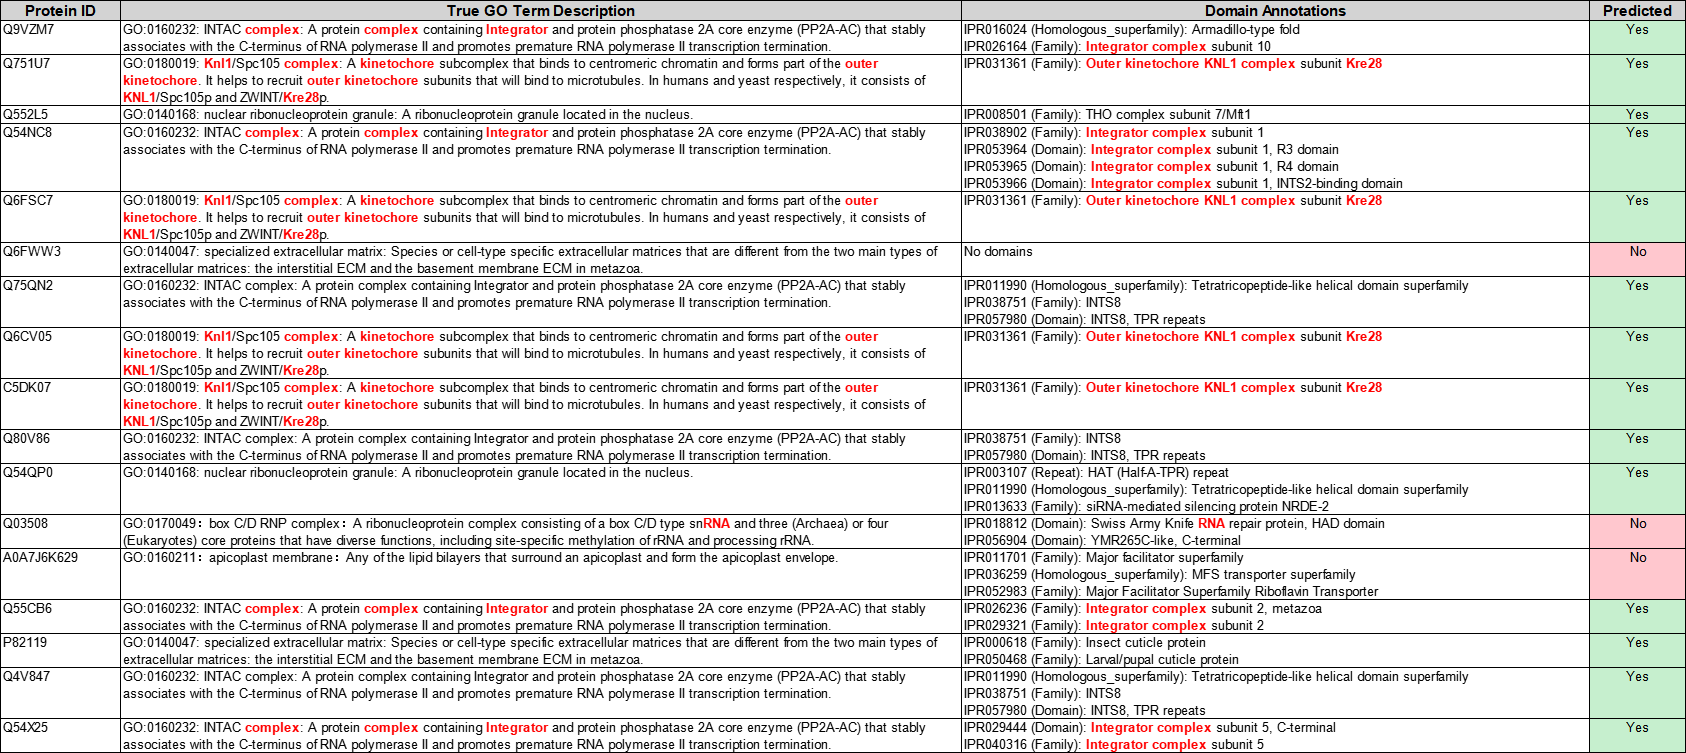
\includegraphics[width=1\linewidth]{picture/cc_text_similarity.png}
    \caption{Case Study of Zero-Shot Predictions in CC Ontology. This table compares the ground truth GO term descriptions with the InterPro domain annotations of the proteins. The "Predicted" column indicates whether MZSGO correctly identified the label.}
    \label{fig:cc_text_sim}
\end{figure}

\newpage
\begin{color}{black}
\section{Extended Ablation Study on BP and MF Ontologies}
\label{supp:ablation_bp_mf}

To further validate the robustness and generalizability of our framework, we extended the ablation study to the BP and MF ontologies. The experimental settings and variant groupings remain identical to those used for the CC ontology described in Section 3.4 of the main text.

The results, presented in Table \ref{tab:ablation_bp} (BP) and Table \ref{tab:ablation_mf} (MF), are highly consistent with our findings on the CC ontology:
\begin{itemize}
    \item \textbf{Necessity of Multimodal Fusion:} Relying on a single modality ("ESM Only" or "Domain Only") leads to a substantial performance drop, particularly in zero-shot metrics (Unseen AUPR and H score).
    \item \textbf{Superiority of Semantic Alignments:} Replacing LLM-based text embeddings with traditional methods ("Domain One-hot" or "PO2Vec Embedding") severely impairs zero-shot performance, reaffirming the importance of deep semantic representations for label understanding.
    \item \textbf{Effectiveness of Architecture:} The "Simple Concat" variant and the "No Feature Drop" setting both underperform compared to MZSGO, proving the necessity of dynamically weighting modalities and utilizing asymmetric feature dropout for regularization.
\end{itemize}

\begin{table}[htbp]
    \centering
    \caption{Ablation experiment results on the Biological Process (BP) ontology.}
    \label{tab:ablation_bp}
    \renewcommand{\arraystretch}{1.1}
    \begin{tabular}{l c c c c c}
        \toprule
        \textbf{Model Variants} & \textbf{Fmax} & \textbf{AUPR} & \textbf{Unseen AUPR} & \textbf{Unseen Fmax} & \textbf{H} \\
        \midrule
        \multicolumn{6}{l}{\textit{Modality Ablation}} \\
        ESM Only & 0.4584 & 0.4278 & 0.0924 & 0.0446 & 0.1520 \\
        Domain Only & 0.4552 & 0.4208 & 0.0774 & 0.0334 & 0.1308 \\
        \midrule
        \multicolumn{6}{l}{\textit{Feature \& Architecture Ablation}} \\
        Domain One-hot & 0.4833 & 0.4550 & 0.2309 & 0.1182 & 0.3066 \\
        Use PO2Vec Embedding & 0.4948 & 0.4721 & 0.0959 & 0.0534 & 0.1595 \\
        No Feature Drop & 0.4992 & 0.4794 & 0.2231 & 0.1440 & 0.3047 \\
        Simple Concat & 0.4849 & 0.4602 & 0.0700 & 0.0352 & 0.1215 \\
        \midrule
        \multicolumn{6}{l}{\textit{Encoder Variants}} \\
        BioGPT & 0.4877 & 0.4650 & 0.1584 & 0.1153 & 0.2364 \\
        BioMedBERT & 0.4829 & 0.4569 & 0.1801 & 0.0931 & 0.2608 \\
        Qwen3-0.6B & 0.4842 & 0.4590 & 0.1964 & 0.0967 & 0.2752 \\
        ESM-150M & 0.4799 & 0.4540 & 0.1730 & 0.1176 & 0.2506 \\
        \midrule
        \multicolumn{6}{l}{\textit{Loss Function Variants}} \\
        Focal Loss & 0.4791 & 0.4787 & 0.1166 & 0.1901 & 0.1876 \\
        BCE (Weighted) & 0.4821 & 0.4580 & 0.1755 & \textbf{0.2141} & 0.2542 \\
        \midrule
        \textbf{MZSGO (Ours)} & \textbf{0.5045} & \textbf{0.5008} & \textbf{0.2393} & 0.1210 & \textbf{0.3250} \\
        \bottomrule
    \end{tabular}
\end{table}

\begin{table}[htbp]
    \centering
    \caption{Ablation experiment results on the Molecular Function (MF) ontology.}
    \label{tab:ablation_mf}
    \renewcommand{\arraystretch}{1.1}
    \begin{tabular}{l c c c c c}
        \toprule
        \textbf{Model Variants} & \textbf{Fmax} & \textbf{AUPR} & \textbf{Unseen AUPR} & \textbf{Unseen Fmax} & \textbf{H} \\
        \midrule
        \multicolumn{6}{l}{\textit{Modality Ablation}} \\
        ESM Only & 0.7322 & 0.6890 & 0.2502 & 0.1516 & 0.3675 \\
        Domain Only & 0.7380 & 0.6986 & 0.4655 & 0.3966 & 0.5598 \\
        \midrule
        \multicolumn{6}{l}{\textit{Feature \& Architecture Ablation}} \\
        Domain One-hot & 0.7376 & 0.7041 & 0.3149 & 0.2367 & 0.4359 \\
        Use PO2Vec Embedding & 0.7414 & 0.7014 & 0.3772 & 0.3871 & 0.4916 \\
        No Feature Drop & 0.7517 & 0.7104 & 0.4800 & 0.4206 & 0.5740 \\
        Simple Concat & 0.7446 & 0.7035 & 0.3951 & 0.3050 & 0.5069 \\
        \midrule
        \multicolumn{6}{l}{\textit{Encoder Variants}} \\
        BioGPT & 0.7506 & 0.7223 & 0.4512 & 0.4290 & 0.5566 \\
        BioMedBERT & 0.7508 & 0.7206 & 0.4513 & 0.4485 & 0.5562 \\
        Qwen3-0.6B & 0.7440 & 0.7111 & 0.3745 & 0.3428 & 0.4915 \\
        ESM-150M & 0.7497 & 0.7202 & 0.4656 & 0.3527 & 0.5667 \\
        \midrule
        \multicolumn{6}{l}{\textit{Loss Function Variants}} \\
        Focal Loss & 0.7280 & 0.6938 & 0.4286 & 0.4835 & 0.5309 \\
        BCE (Weighted) & 0.7372 & 0.7074 & \textbf{0.5526} & \textbf{0.5585} & \textbf{0.6234} \\
        \midrule
        \textbf{MZSGO (Ours)} & \textbf{0.7611} & \textbf{0.7337} & 0.4806 & 0.4259 & 0.5821 \\
        \bottomrule
    \end{tabular}
\end{table}
\end{color}

\newpage
\section{Analysis of Adaptive Gate Weights}

To understand how MZSGO integrates multimodal information, we analyzed the average gate weights assigned to Domain ($\alpha$), ESM sequence ($\beta$), and NLP text ($\gamma$) features across the three GO ontologies. The gate weights are dynamically learned, reflecting the model's reliance on specific modalities for different prediction tasks. Figure \ref{fig:gate_weights} illustrates the weight distribution across Overall, Unseen, Seen, and Zero-shot specific label sets.

Consistent with the ablation results in Section 3.4, CC exhibits a heavy reliance on Domain features, with an average weight of 83.60\% overall, rising to 91.23\% for unseen labels. This suggests that subcellular localization is strongly correlated with specific protein domains and motifs, which provide more generalizable signals than raw sequences for this ontology. In contrast, for BP, the model prioritizes ESM sequence features for seen labels (53.66\%), likely because sequence homology is a strong predictor for known functions. However, a significant shift occurs for ``Zero'' labels (labels with very few or no training samples), where the model increases its reliance on Domain features (from 31.11\% overall to 44.76\%) and NLP features. This adaptive shift demonstrates MZSGO's ability to leverage semantic domain descriptions when sequence patterns alone are insufficient for rare or novel classes. Finally, MF shows a more balanced distribution between Domain ($\sim$48\%) and ESM ($\sim$48\%) features, indicating that enzymatic activities and binding functions require both the structural cues provided by domains and the fine-grained residue information captured by the ESM encoder. Overall, the gate weight analysis confirms that MZSGO does not simply average modalities but adaptively selects the most informative representation based on the ontology and the specific nature (seen vs. unseen) of the target labels.

\begin{figure}[htbp]
    \centering
    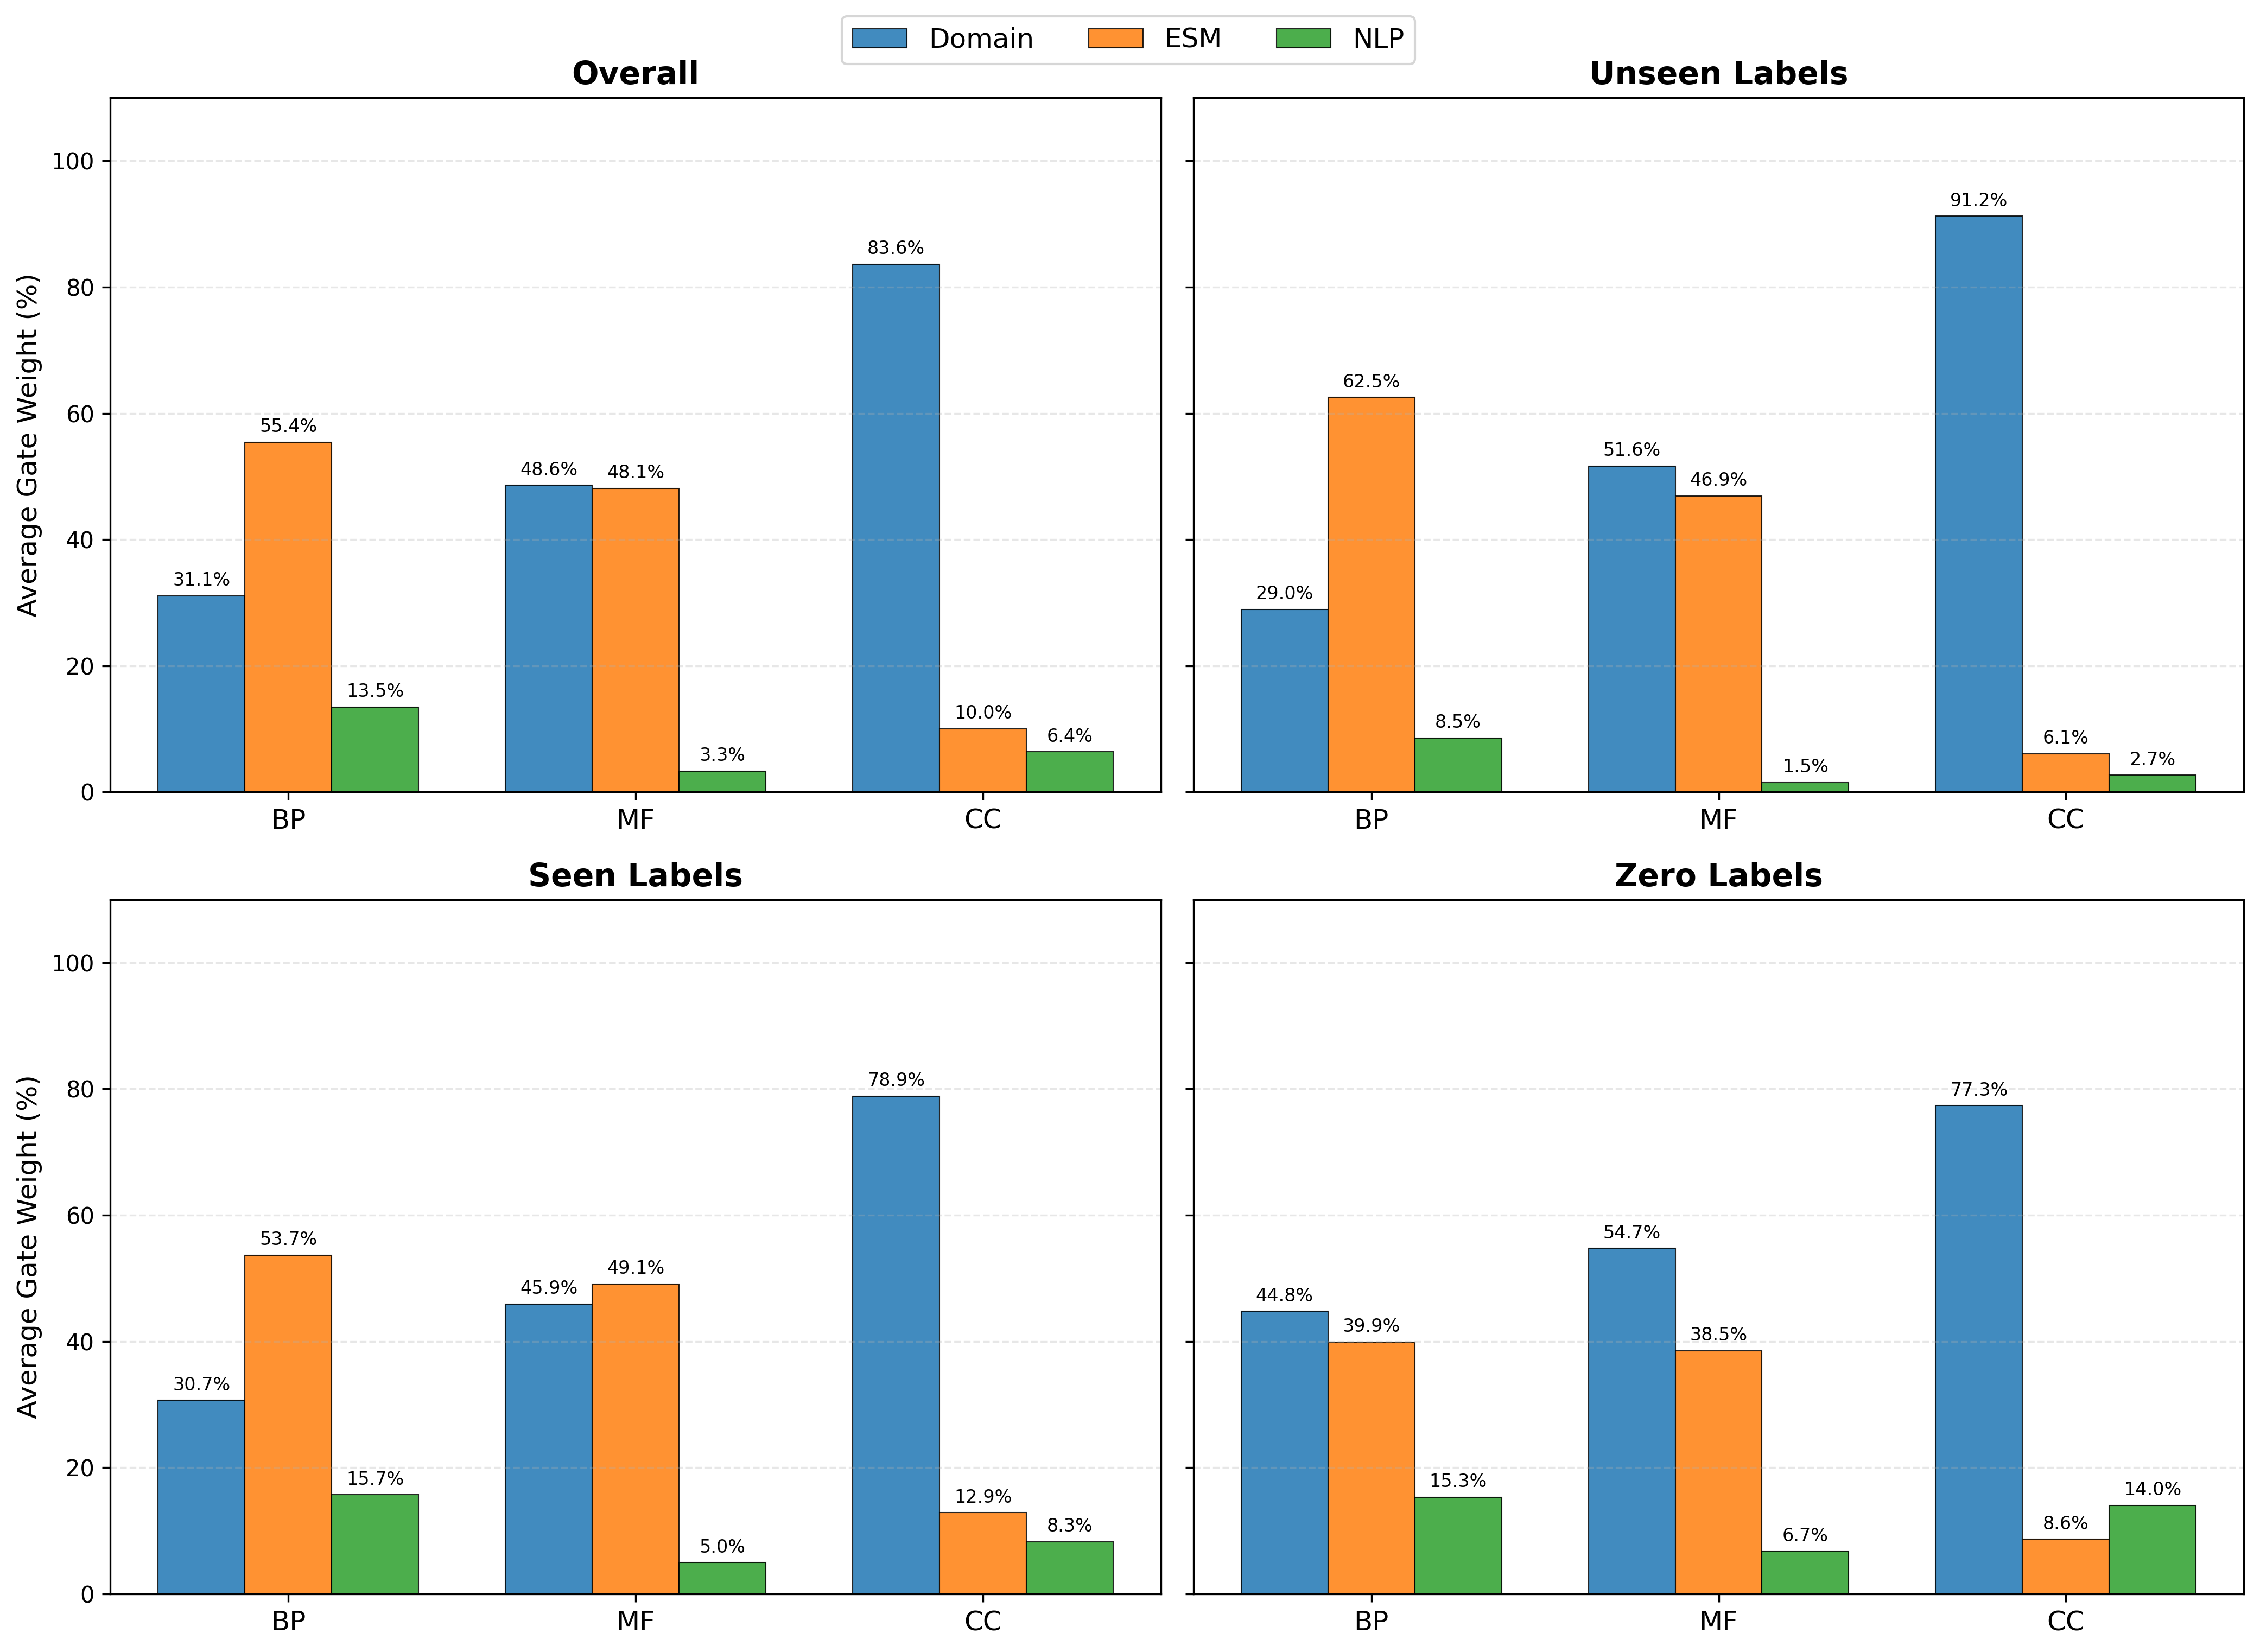
\includegraphics[width=0.8\linewidth]{picture/gate_weights_analysis.png} 
    \caption{Comparison of adaptive gate weights assigned to Domain, ESM, and NLP modalities across BP, MF, and CC. The subplots show distributions for Overall data, Unseen labels, Seen labels, and Zero-shot labels.}
    \label{fig:gate_weights}
\end{figure}

\newpage
\begin{color}{black}

\section{Impact of Hierarchical Consistency and True Path Rule}
\label{supp:tpr}

Gene Ontology (GO) terms are structured as a Directed Acyclic Graph (DAG), which implies the \textit{True Path Rule} (TPR)\cite{notaro2021hemdag}: if a protein is annotated with a specific term, it must also be annotated with all its ancestral terms. Conversely, if a protein is not annotated with a term, it cannot be annotated with any of its descendant terms. 

\subsection{Implementation of Hierarchical Propagation}
To evaluate whether explicit hierarchical constraints enhance the performance of MZSGO, we implemented a post-processing propagation mechanism, denoted as \textbf{MZSGO\_PROP}. Given the raw prediction scores $S$ for a protein across $L$ labels, we ensure hierarchical consistency by propagating the maximum scores from children to parents according to the DAG structure:
\begin{equation}
    S_{p}^* = \max \left( S_p, \max_{c \in \text{children}(p)} S_c \right)
\end{equation}
where $S_p$ is the original score for a parent term and $S_{p}^*$ is the corrected score. This ensures that the prediction score of a parent term is always greater than or equal to the score of any of its descendants.

\subsection{Experimental Results and Discussion}
We compared the performance of the original MZSGO (separate training for each ontology) with MZSGO\_PROP. The results across Biological Process (BP), Molecular Function (MF), and Cellular Component (CC) are summarized in Table \ref{tab:tpr_results}.

\begin{table}[htbp]
    \centering
    \caption{Performance comparison between the original MZSGO and MZSGO with True Path Rule propagation (MZSGO\_PROP). The metrics include overall Fmax and AUPR, as well as AUPR for Seen/Unseen labels and the Harmonic Mean (H).}
    \label{tab:tpr_results}
    \small
    \begin{tabularx}{\textwidth}{l l c c c c c}
        \toprule
        \textbf{Ontology} & \textbf{Model} & \textbf{Fmax} $\uparrow$ & \textbf{AUPR} $\uparrow$ & \textbf{Unseen AUPR} $\uparrow$ & \textbf{Seen AUPR} $\uparrow$ & \textbf{H} $\uparrow$ \\
        \midrule
        \multirow{2}{*}{BP} & MZSGO & 0.5045 & 0.5008 & 0.2393 & 0.5021 & 0.3241 \\
         & MZSGO\_PROP & \textbf{0.5066} & \textbf{0.5046} & \textbf{0.2394} & \textbf{0.5060} & \textbf{0.3250} \\
        \midrule
        \multirow{2}{*}{MF} & MZSGO & 0.7611 & 0.7337 & \textbf{0.4806} & 0.7380 & 0.5821 \\
         & MZSGO\_PROP & \textbf{0.7628} & \textbf{0.7356} & \textbf{0.4806} & \textbf{0.7399} & \textbf{0.5827} \\
        \midrule
        \multirow{2}{*}{CC} & MZSGO & 0.7470 & 0.7726 & \textbf{0.5862} & 0.7733 & 0.6669 \\
         & MZSGO\_PROP & \textbf{0.7482} & \textbf{0.7736} & \textbf{0.5862} & \textbf{0.7743} & \textbf{0.6672} \\
        \bottomrule
    \end{tabularx}
\end{table}

As observed in Table \ref{tab:tpr_results}, the integration of explicit TPR propagation leads to marginal improvements (e.g., $<0.3\%$ in Fmax) across all three ontologies. This finding suggests that MZSGO's multi-modal matching mechanism is inherently capable of capturing hierarchical dependencies. By leveraging LLM-based embeddings of GO definitions, the model learns a latent space where semantically (and thus hierarchically) related terms are positioned closely, naturally leading to consistent score assignments without the need for rigid architectural constraints or complex post-processing.
\end{color}

\bibliographystyle{plain}
\bibliography{reference} 

\end{document}